\begin{figure}
   \begin{subfigure}[t]{0.48\textwidth}
      \begin{nscenter}
         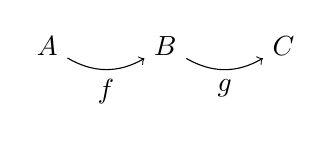
\begin{tikzpicture}[node distance=1.5cm, auto]
            \node (A) [node distance=2cm] {
               $A$
            };
            \node (B) [right of=A] {
               $B$
            };
            \node (C) [right of=B] {
               $C$
            };
            \draw[->, bend right] (A) to node [swap] {$\lowerAdj{f}$} (B);
            \draw[->, bend right] (B) to node [swap] {$\upperAdj{g}$} (C);
         \end{tikzpicture}
      \end{nscenter}
   \end{subfigure}
   \begin{subfigure}[t]{0.48\textwidth}
      \begin{nscenter}
      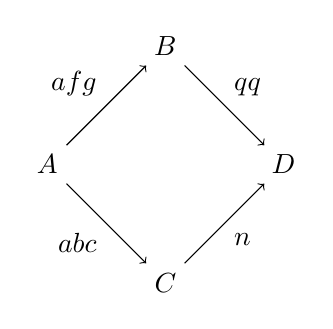
\begin{tikzpicture}[node distance=1.5cm, auto]
      \node (P) [node distance=2cm] {
         $A$
      };
      \node (R) [right of=P, above of=P] {
         $B$
      };
      \node (RPrime) [below of=P, right of=P] {
         $C$
      };
      \node (PPrime) [right of=R, below of=R] {
         $D$
      };
      \draw[->] (P) to node {$afg$} (R);
      \draw[->] (P) to node [swap] {$abc$} (RPrime);
      \draw[->] (R) to node {$qq$} (PPrime);
      \draw[->] (RPrime) to node [swap] {$n$} (PPrime);
      \end{tikzpicture}
   \end{nscenter}
\end{subfigure}
\caption{Inverting a Galois connection using De Morgan duality}
\end{figure}
